\section{\printdate{2015/08/24} - Building GEOtop on OS X}\label{sec:20150824}

In order to build GEOtop on OS X, it's necessary to have a package manager installed. Several package managers are available:

\begin{itemize}
\item MacPorts;
\item Fink;
\item Homebrew.
\end{itemize}
The last one is the newest and most popular of the trio. So, because I'm working on \textbf{Yosemite 10.10.5}, I followed this guide \url{http://coolestguidesontheplanet.com/installing-homebrew-os-x-yosemite-10-10-package-manager-unix-apps/} to install it.

\subsection{Building master-branch: shared linking}

\begin{itemize}
\item \textcolor{blue}{PROJ4 and BOOST}\newline In case of dynamic linking, the precompiled packages of the libraries \textbf{PROJ4} and \textbf{BOOST} may been installed through the package manager.

\begin{lstlisting}[style=bashStyle]
$ brew search proj
$ brew install proj

# necessary to create symlink in /usr/local/lib to the PROJ4 shared and static libraries which have to be found and linked at run-time
$ brew link --overwrite proj
$ brew search boost
$ brew install boost boost-build
\end{lstlisting} %$

\item \textcolor{blue}{MeteoIO 2.4.2} (\url{http://models.slf.ch/p/meteoio/downloads/})\newline The MeteoIO library has to be compiled.
\newline\textsc{\textcolor{red}{=> REMEMBER 1:} GEOtop can be built only against MeteoIO 2.4.2.}
\newline\textsc{\textcolor{red}{=> REMEMBER 2:} Download the source code, no precompiled versions.}

You can get the source code downloading it from the website, or through the \inline{wget} command.

\begin{lstlisting}[style=bashStyle]
# install wget, it's not installed by default in OS X
$ brew install wget

# download the source code in the preferred directory
$ wget http://models.slf.ch/p/meteoio/downloads/get/MeteoIO-2.4.2-src.tar.gz

# extract source code from tar file
$ tar -xzvf MeteoIO-2.4.2-src.tar.gz

# cd into the MeteoIO working directory
$ cd MeteoIO-2.4.2/
\end{lstlisting}
The next step is building the source code. It's rather easy, but first of all you have to install the building system: \textbf{CMake}.

\begin{lstlisting}[style=bashStyle]
$ brew search cmake
$ brew install cmake
\end{lstlisting}
The following steps are strictly related to the building part.

\begin{lstlisting}[style=bashStyle]
$ ccmake .
\end{lstlisting} %$

\begin{figure*}[h]
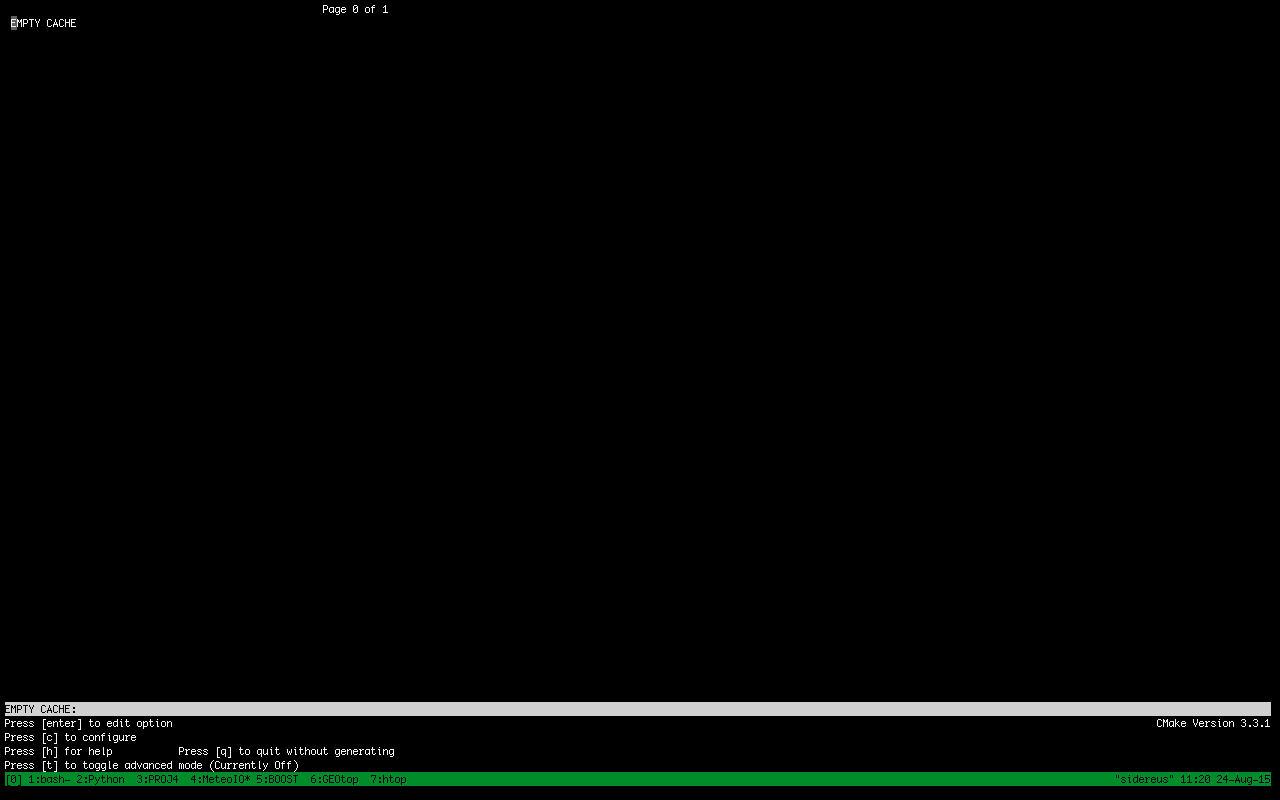
\includegraphics[width=\linewidth]{2015/Aug/24/1pic.png}
\end{figure*}

\pagebreak

\begin{lstlisting}[style=bashStyle]
# then press 'c' to configure
\end{lstlisting}

\begin{figure*}[h]
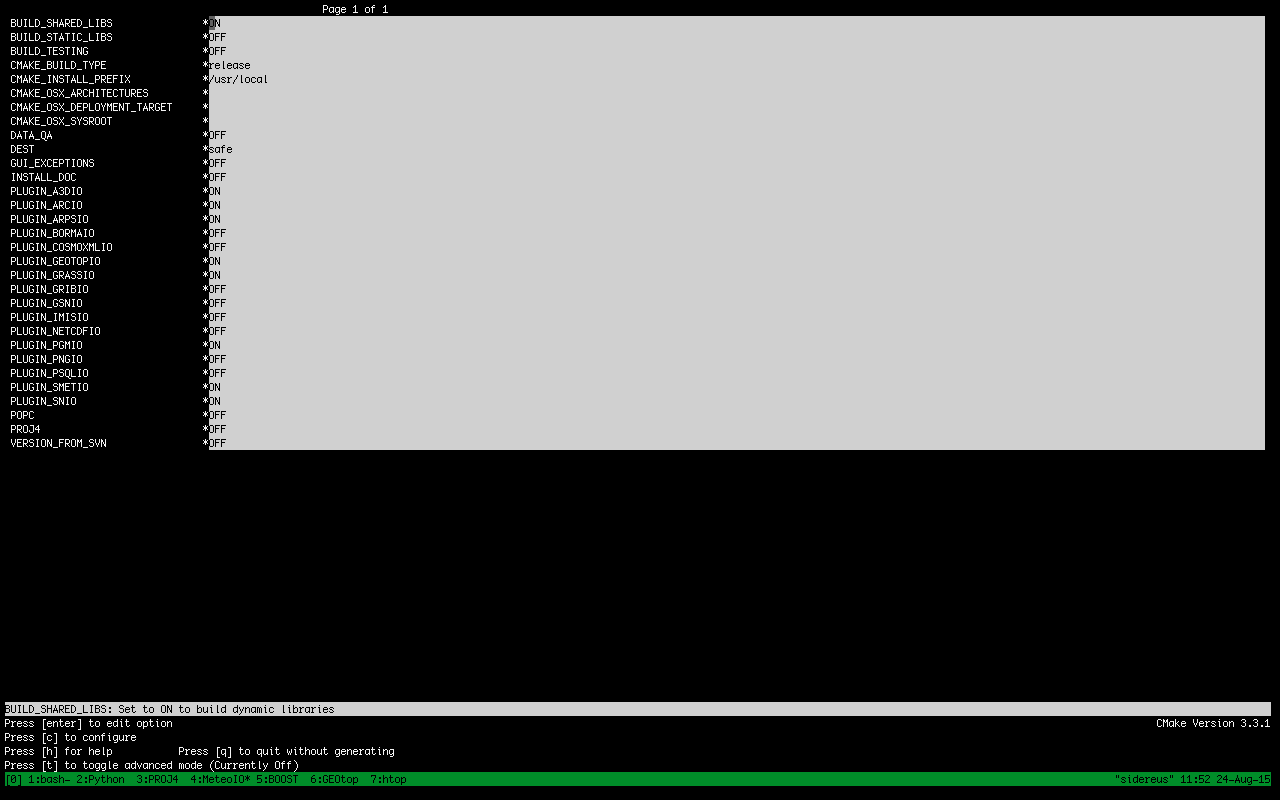
\includegraphics[width=\linewidth]{2015/Aug/24/2pic.png}
\end{figure*}

\pagebreak

\begin{lstlisting}[style=bashStyle]
# go to the last of one line and change PROJ4 flag: OFF => ON
\end{lstlisting}

\begin{figure*}[h]
  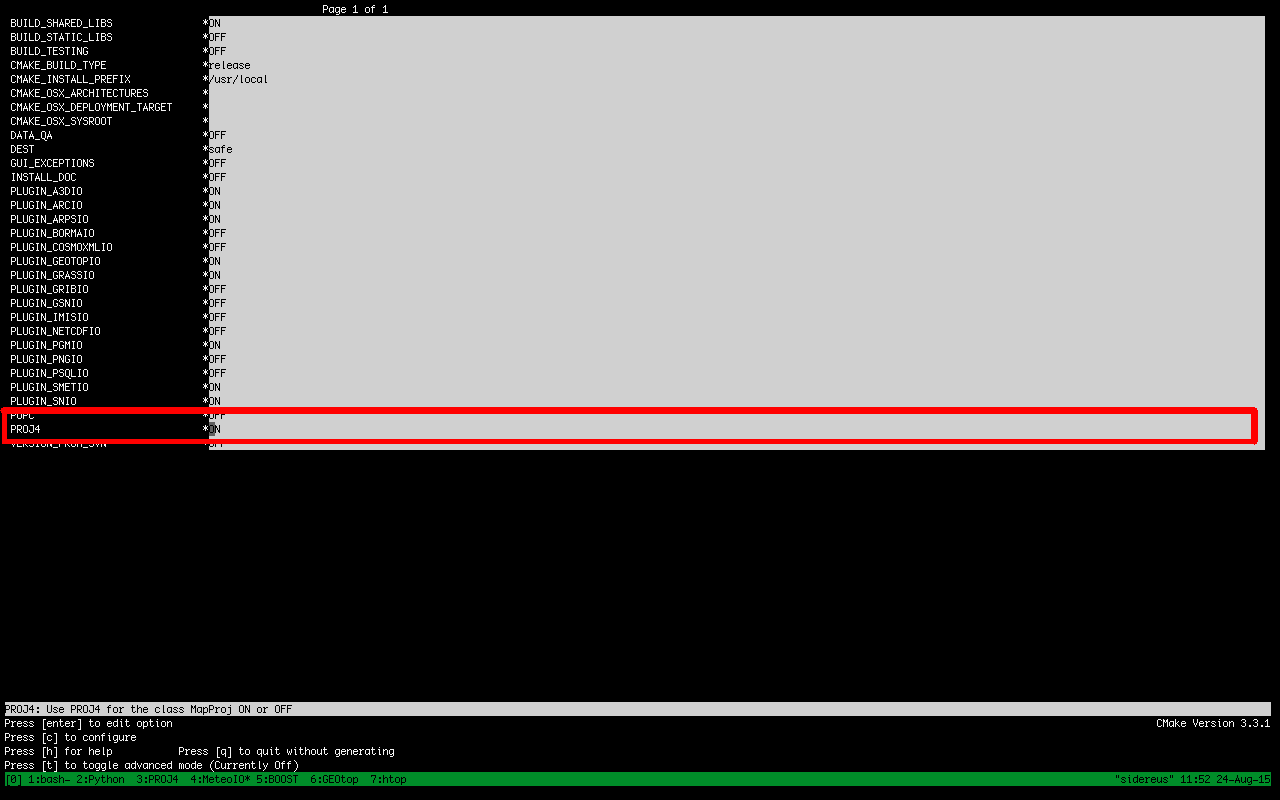
\includegraphics[width=\linewidth]{2015/Aug/24/3pic.png}
\end{figure*}

\pagebreak

\begin{lstlisting}[style=bashStyle]
# then press 'c' to configure
\end{lstlisting}

\begin{figure*}[h]
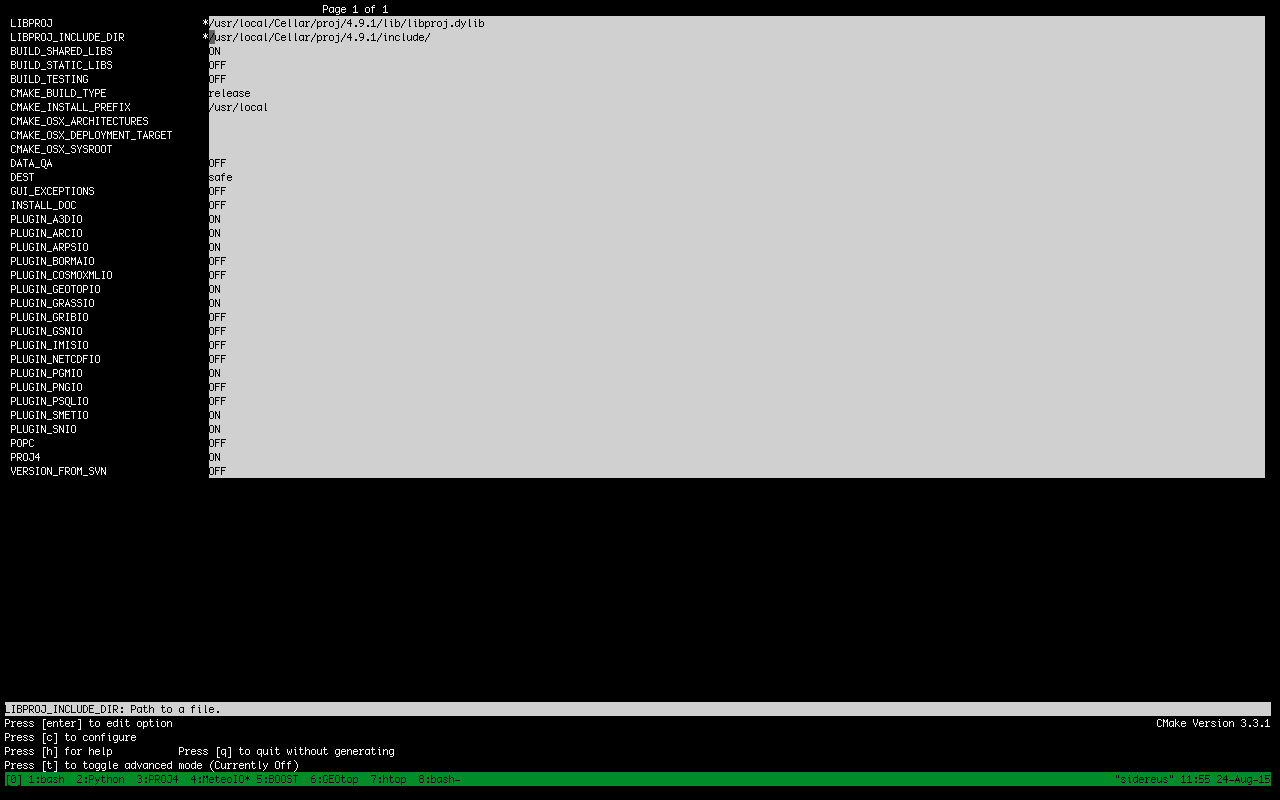
\includegraphics[width=\linewidth]{2015/Aug/24/7pic.png}
\end{figure*}

\pagebreak

\begin{lstlisting}[style=bashStyle]
# press 'c' to configure and the 'g' to generate
# after pressing 'g' you might have got a warning message but this depends on your cmake version and it's not a problem. in this case you just have to press 'e' to exit as well
\end{lstlisting}

\begin{figure*}[h]
  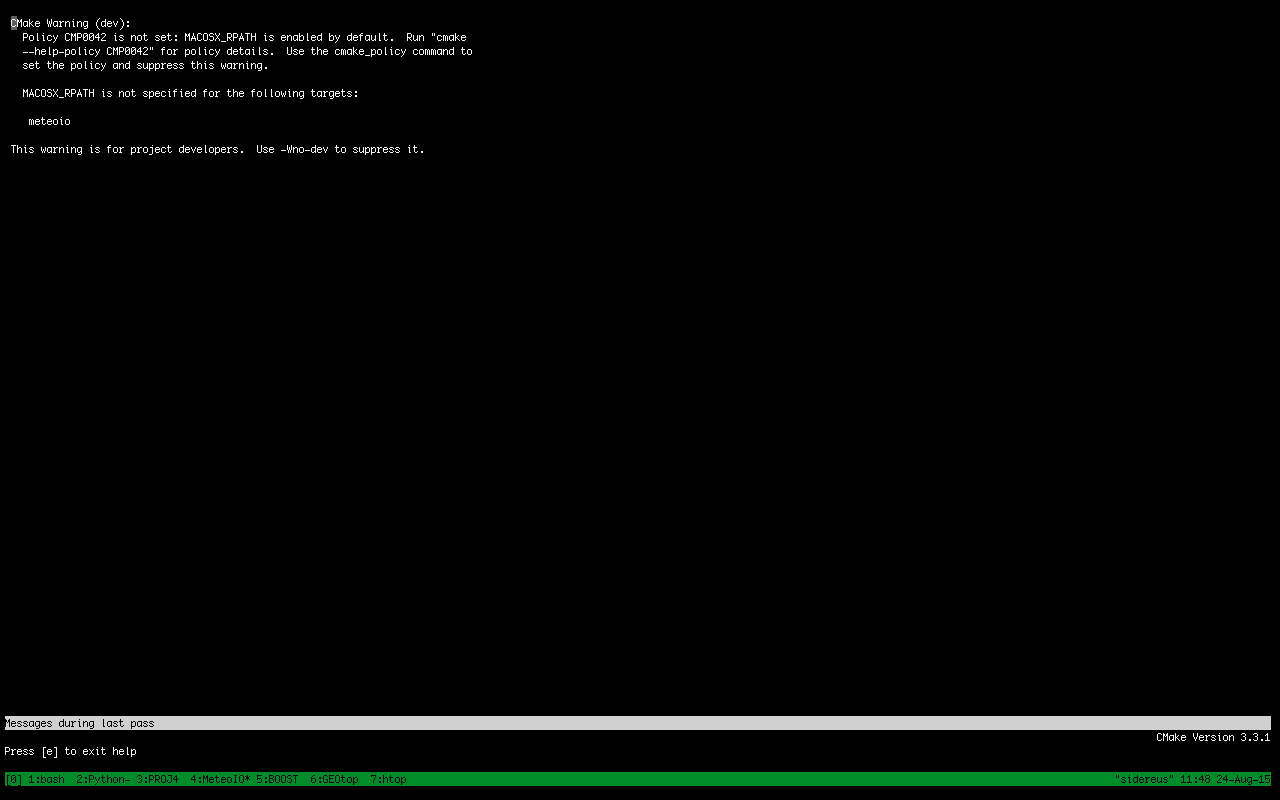
\includegraphics[width=\linewidth]{2015/Aug/24/8pic.png}
\end{figure*}

\begin{lstlisting}[style=bashStyle]
$ make
# if everything is ok
$ make install
# otherwise write to geotopusers@googlegroups.com adding the resulting error
\end{lstlisting}

\item \textcolor{blue}{GEOtop}
  You can get the source code cloning it from a GitHub repository. You might need to install \inline{git} version control system. So

\begin{lstlisting}[style=bashStyle]
$ brew search git
$ brew install git
$ cd into/directory/to/save/GEOtop/src/
$ git clone https://github.com/francescoS/geotop
# cd into the GEOtop working directory
$ cd geotop/
\end{lstlisting} %$

The next step is building the source code. It's quite similar to building MeteoIO.

\pagebreak

\begin{lstlisting}[style=bashStyle]
$ ccmake .
\end{lstlisting} %$

\begin{figure*}[h]
  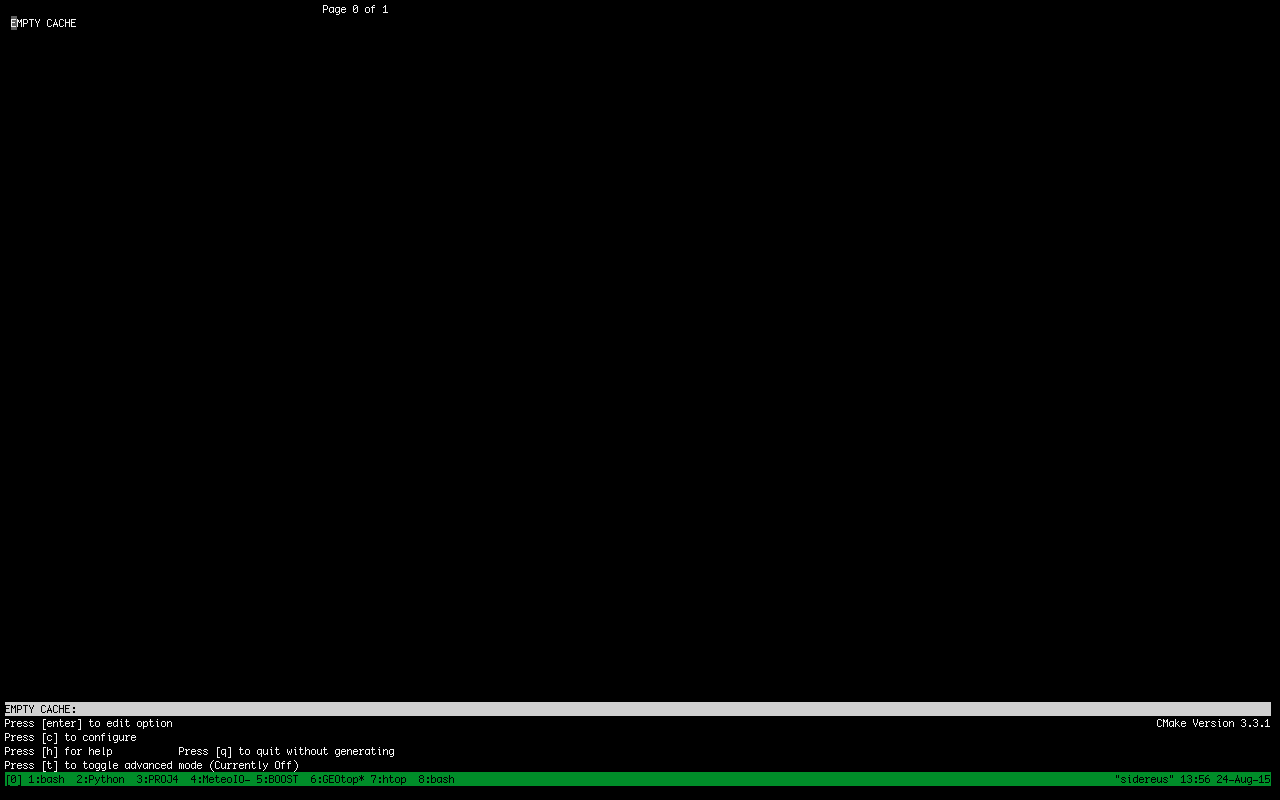
\includegraphics[width=\linewidth]{2015/Aug/24/1picGT.png}
\end{figure*}

\pagebreak

\begin{lstlisting}[style=bashStyle]
# press 'c' to configure
# the linking library mode is shown (in this specific case SHARED)
# press 'e' to exit
\end{lstlisting}

\begin{figure*}[h]
  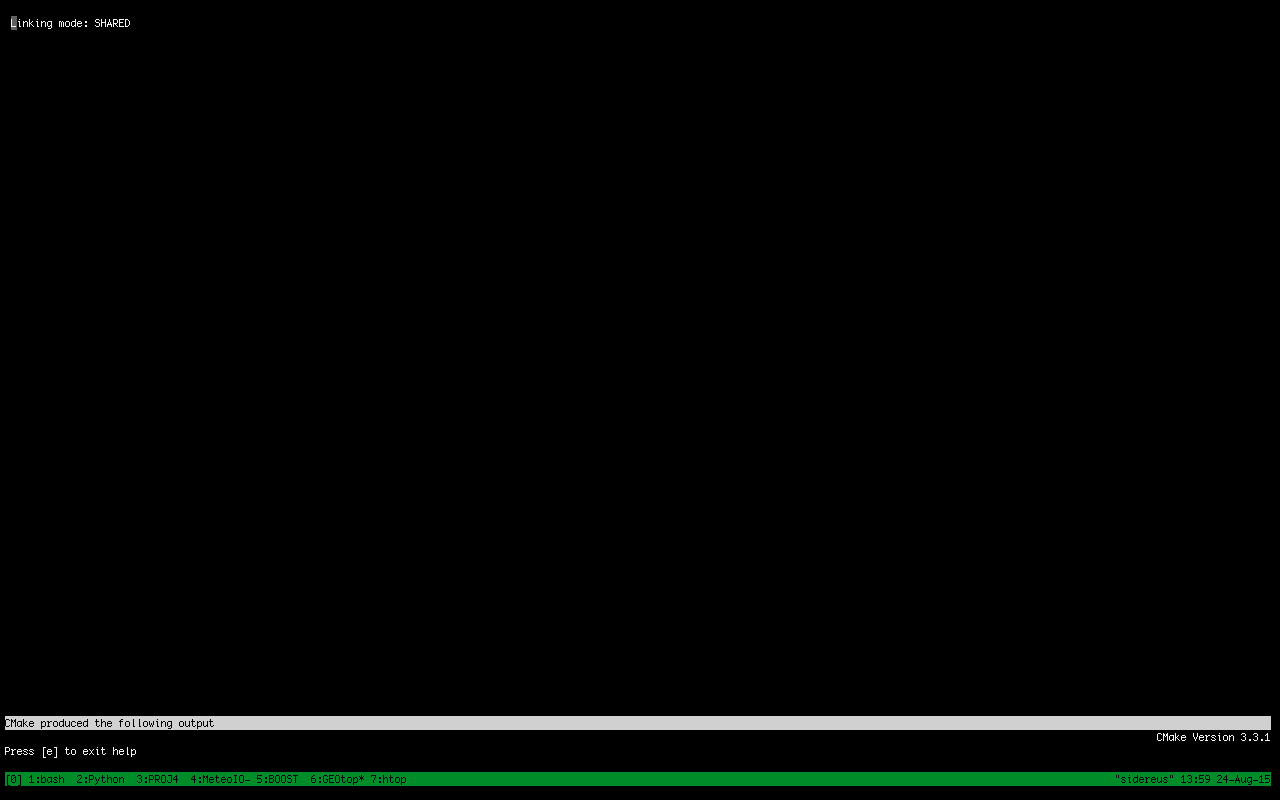
\includegraphics[width=\linewidth]{2015/Aug/24/2picGT.png}
\end{figure*}

\pagebreak

Now you have to do an important choice: using MeteoIO interpolation or GEOtop internal routines. To do that

\begin{itemize}
\item \inline{ENABLE_INTERNAL_METEODISTR} $\qquad$ \inline{ON}\newline use GEOtop internal routines;
\item \inline{ENABLE_INTERNAL_METEODISTR} $\qquad$ \inline{OFF}\newline use MeteoIO time and space interpolation.
\end{itemize}

\begin{figure*}[h]
  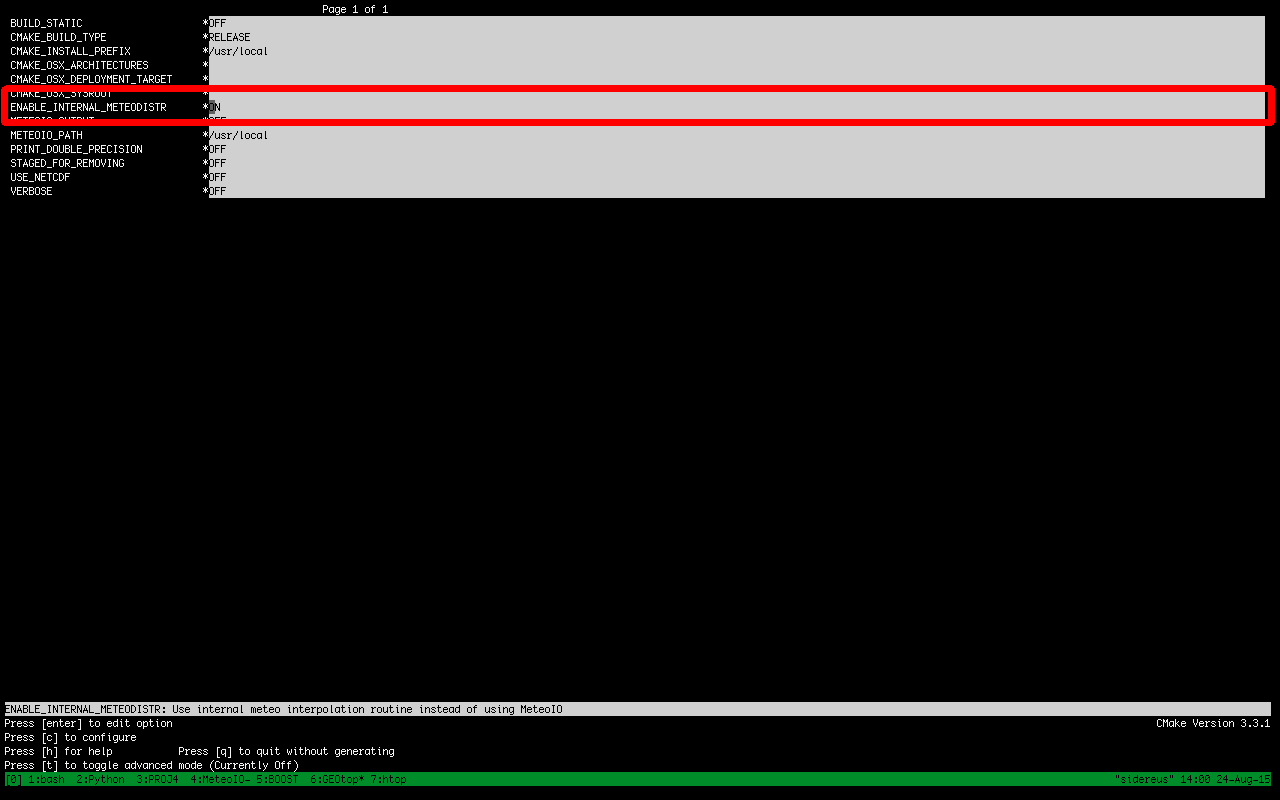
\includegraphics[width=\linewidth]{2015/Aug/24/3picGT.png}
\end{figure*}

\pagebreak

\begin{figure*}[h]
  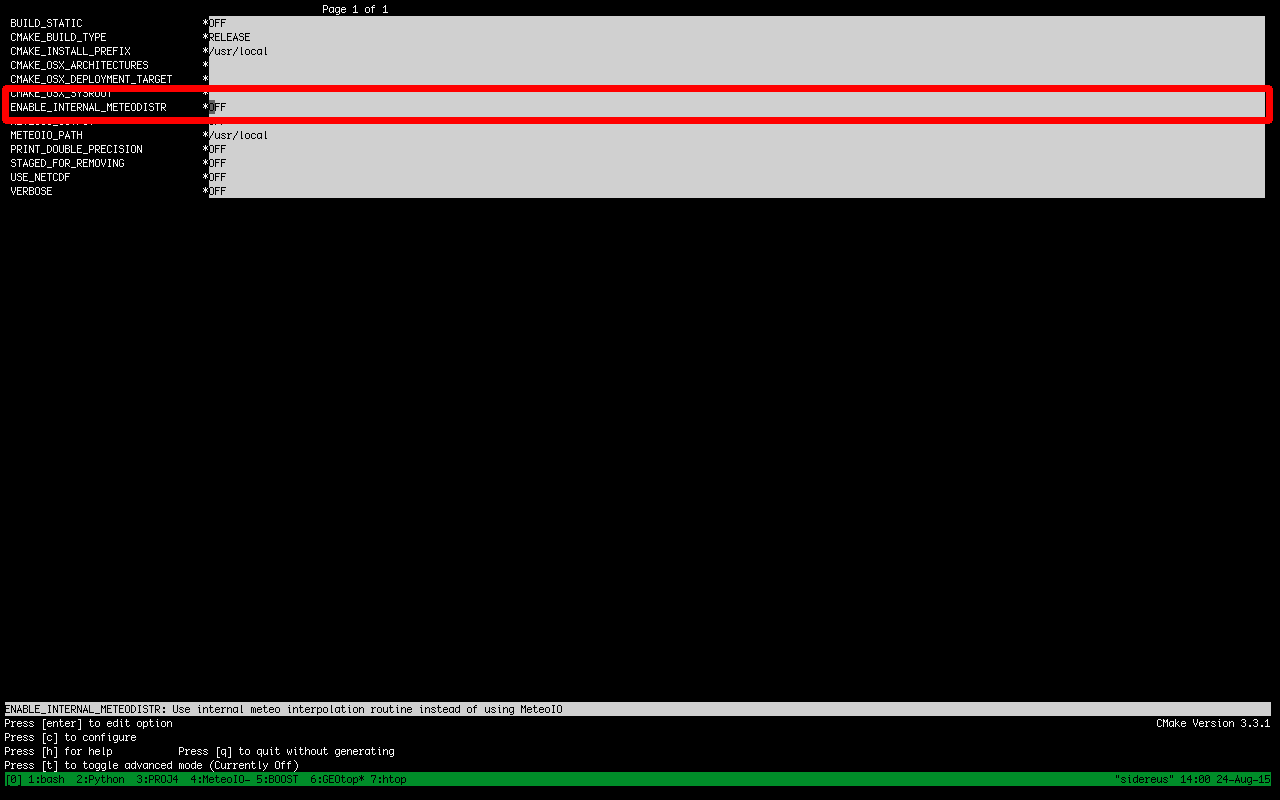
\includegraphics[width=\linewidth]{2015/Aug/24/4picGT.png}
\end{figure*}

\begin{lstlisting}[style=bashStyle]
# press 'c' to configure
# press 'e' to exit
# press 'g' to generate
\end{lstlisting}

\pagebreak

\begin{lstlisting}[style=bashStyle]
# you might get a warning. It doesn't matter, press 'e' to exit and go on
\end{lstlisting}

\begin{figure*}[h]
  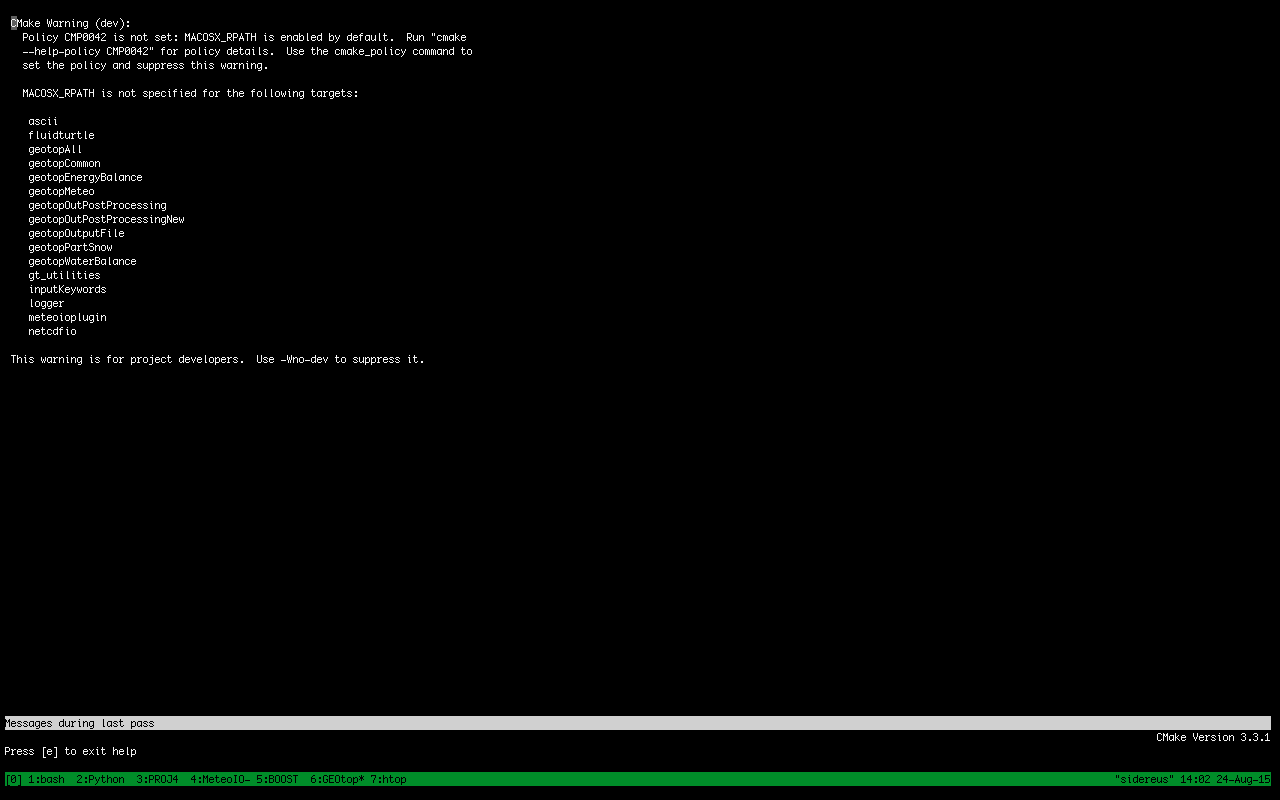
\includegraphics[width=\linewidth]{2015/Aug/24/5picGT.png}
\end{figure*}

\begin{lstlisting}[style=bashStyle]
$ make
# if everything is ok enjoy the powerful of the GEOtop model
# otherwise write to geotopusers@googlegroups.com adding the resulting error
\end{lstlisting} %$
  
\end{itemize}

\subsection{Building master-branch: static linking}

The building of the master-branch in \textbf{static linking mode} doesn't work.

\subsection{Building cmake\_redesign-branch: shared linking}

\textsc{\textcolor{red}{=> WIN} (What Is New):} the work done in this branch has been described in \printdate{2015/06/24}, \printdate{2015/07/14} and \printdate{2015/07/15}. The main news is the possibility of installing the GEOtop binary, so that you can just call

\begin{lstlisting}[style=bashStyle]
$ geotop /path/of/working/directory
\end{lstlisting} %$

Compared to what previously designed, an important bug has been fixed: the declaration of the variables of the internal libraries in the CMake script has been moved from \inline{src/geotop/CMakeLists.txt} to \inline{src/CMakeLists.txt}.

This branch is going to be merged in a few weeks, anyway building this source code is like building it on the master branch. Before starting the procedure you have to switch branch, once have changed directory into the GEOtop working directory.

\begin{lstlisting}[style=bashStyle]
$ git checkout cmake_redesign
\end{lstlisting} %$

Then follow the building instructions; at the end of the procedure just type

\begin{lstlisting}[style=bashStyle]
$ make install
\end{lstlisting} %$

to get a working GEOtop binary file from within every point of your local disk.

\subsection{Building cmake\_redesign-branch: static linking}